%%Sorting Networks File. 

%Intro subsection
\section{Sorting Networks}
Let a \emph{wire} be a horizontal line. Let a \emph{comparator} be a vertical line connecting two wires. A 
\emph{sorting network} is a device consisting of $[1 \dots n]$ wires and $[0 \dots m]$  
comparators such that the sorting network sorts a permutation of $n$ elements into ascending order. The 
$n$ elements are first listed to the left of each wire in the network. The elements travel across their respective wires 
at the same time. When a pair of elements, traveling through a pair of wires, 
encounter a comparator, the comparator swaps the elements if and only if the top wire's element 
is greater than the bottom wire's element. A sorting network with $n$ wires and $m$ 
comparators that can sort any permutation of order $n$ is a \emph{complete sorting network}. 
To see a complete sorting network for $n=4$ please refer to Figure~\ref{Fig:SortNetwork}.\par 

\begin{figure}[h]
   ~\centering
    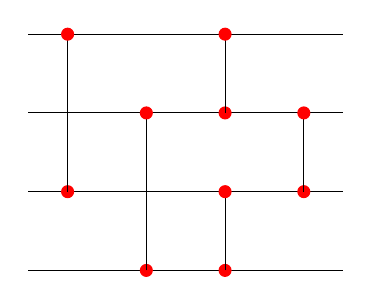
\begin{tikzpicture}
        \draw(0, 0) to (4, 0);
           
        \draw(0, 1) to (4, 1);
        \draw(0, 2) to (4, 2);
           
        \draw(0, 3) to (4, 3);

        %%connector 1
        \draw[red, fill=red](.5,1) circle (.5ex);
            \draw(.5, 1) to (.5, 3);
        \draw[red, fill=red](.5,3) circle (.5ex);


        %%connector 2 
        \draw[red, fill=red](1.5,0) circle (.5ex);
            \draw(1.5, 0) to (1.5, 2);
        \draw[red, fill=red](1.5,2) circle (.5ex);

        %%connector 3
        \draw[red, fill=red](2.5,2) circle (.5ex);
            \draw(2.5, 2) to (2.5, 3);
        \draw[red, fill=red](2.5,3) circle (.5ex);

        \draw[red, fill=red](2.5,0) circle (.5ex);
            \draw(2.5, 0) to (2.5, 1);
        \draw[red, fill=red](2.5,1) circle (.5ex);
        
        %%connector 4
        \draw[red, fill=red](3.5,1) circle (.5ex);
            \draw(3.5, 1) to (3.5, 2);
        \draw[red, fill=red](3.5,2) circle (.5ex);


    \end{tikzpicture}
    \caption{Complete Sorting Network for $n=4$.}
    \label{Fig:SortNetwork}
\end{figure}

Sorting networks were first studied in 1954 by Armstrong, Nelson and O'Connor~\cite{A18}. 
Donald Knuth describes how the comparators for binary integers can be implemented as simple, 
three-state electronic devices~\cite{A18}. Batcher, in 1968, 
suggested using them to construct switching networks for computer hardware, replacing 
both buses and the faster, but more expensive, crossbar switches~\cite{A27}. Currently, sorting networks 
are implemented in graphical processing units, GPUs, for faster sorting methods than traditional CPU sorting methods~\cite{A28}.\par  
Let a \emph{minimum sorting network} be defined 
as a sorting network such that for any arbitrary comparator, $c$, on wire $i$, $c$ connects to line $i+1$ or $i-1$. Furthermore, 
the number of comparators in a minimum sorting network is equal to the number of inversions in $\pi$. Clearly, there is a 
bijection from comparators in a minimum sorting network to the bars in an optimal ladder lottery, and there 
is a bijection from the wires in a minimum sorting network and the lines in a ladder lottery. 


 
\subsection{The Integer Sequence Relating to the Reverse Permutation}
Let $\pi=(n,n-1, \dots 2,1)$ refer to the reverse permutation order $n$. 
There is an integer sequence that counts the number of minimum sorting networks 
for $\pi$. This integer sequence also counts $OptL\{(n,n-1, \dots 2,1)\}$. This sequence grows very quickly, therefore $n=15$ 
is  the largest value this integer sequence has been calculated for. To refer to the table for this sequence 
please refer to Table~\ref{Tab:IntSeq1}~\cite{A30}.
\begin{table}[t]
    \begin{center}

    \begin{tabular}{|p{2cm}||p{8cm}|}
        \hline
        \multicolumn{2}{|c|}{Number of minimum sorting networks/$|OptL\{Rev(\pi)\}|$}\\
        \hline
        n & Count \\ 
        \hline 
        1 & 1 \\
        \hline 
        2 & 1 \\
        \hline 
        3 & 2 \\
        \hline 
        4 & 8 \\
        \hline 
        5 & 62 \\
        \hline 
        6 & 908 \\
        \hline 
        7 & 24698 \\
        \hline 
        8 & 1232944 \\
        \hline 
        9 & 112018190 \\
        \hline 
        10 & 18410581880 \\
        \hline 
        11 & 5449192389984 \\ 
        \hline 
        12 & 2894710651370536 \\
        \hline 
        13 & 2752596959306389652 \\
        \hline 
        14 & 4675651520558571537540 \\
        \hline 
        15 & 14163808995580022218786390 \\
        \hline 
    \end{tabular}
    \end{center}
    \caption{Number of minimum sorting networks and $|OptL\{Rev(\pi)\}|$}
    \label{Tab:IntSeq1}
\end{table}\par
Dumitrescu and Mandal, in their paper New Lower Bounds For The Number of Pseudoline Arrangements~\cite{A33}
published in 2018, provide the current best known lower bound for this sequence as  
$bn \geq cn^{2} - O(n log n)$ for some constant $c > 0.2083$. In particular, $bn \geq 0.2083 n^{2}$
for large values of $n$. Where $bn$ is the bound for a given value $n$. In the paper, Coding 
and Counting Arrangements of Pseudolines~\cite{A32} by Felsner and Valtr, written in 2011, the authors demonstrate 
the best known upper bound for this sequence is $bn \leq 2^{0.657n^{2}}$.\par 

Seeing as there is yet to be a closed form solution for this sequence, new values of $n$ are counted by a variety of algorithms. 
In the paper, Efficient Enumeration of all Ladder Lotteries and its Application~\cite{A1}, 
the authors were the first to calculate the sequence for $n=11$ with the algorithm {\sc FindAllChildren}. 
In the paper, Counting Primitive Sorting Networks by $\mathbb{\pi}$DDs~\cite{A29}, written by Kawahara, Minato, Saitoh and Yoshinaka, the authors
 were the first to calculate for $n=13$ with a data structure they have termed $\mathbb{\pi}$DD.
\pagebreak



